\chapter{Kết quả thực nghiệm và đánh giá}

Chương này trình bày kết quả triển khai các chức năng chính, thực nghiệm Virtual Try-On và đánh giá những quyết định kiến trúc của hệ thống. Phần thực nghiệm tập trung vào khả năng tạo ảnh thử đồ và thời gian xử lý của CatVTON cục bộ so với FLUX.2 qua Replicate trên cùng bộ ảnh đầu vào.

\medskip

\section{Kết quả triển khai chức năng}

Các luồng chức năng được kiểm tra từ giao diện người dùng tới hệ thống nghiệp vụ và dịch vụ AI. Kết quả tổng hợp trong Bảng~\ref{tab:functional-results} cho thấy hệ thống đã hiện thực được chuỗi tương tác chính của một nền tảng thương mại điện tử thời trang tích hợp AI.

\medskip

\begin{table}[H]
\centering
\small
\caption{Kết quả kiểm tra các chức năng chính}
\label{tab:functional-results}
\begin{tabularx}{\textwidth}{L{3.2cm}L{3.0cm}Y}
\toprule
\textbf{Chức năng} & \textbf{Kết quả} & \textbf{Minh chứng triển khai} \\
\midrule
Cửa hàng và giỏ hàng & Đạt phạm vi tối thiểu & Hiển thị sản phẩm từ Medusa Store API, tìm kiếm, sắp xếp, thêm sản phẩm và thay đổi số lượng. \\
\addlinespace
Hồ sơ AI và tủ đồ & Đạt phạm vi tối thiểu & Lưu ảnh cơ thể và thông tin hồ sơ; thêm, hiển thị và xóa trang phục cá nhân. \\
\addlinespace
AI Stylist & Hoàn thành luồng chính & Phân tích yêu cầu, truy hồi dữ liệu từ LanceDB, sinh phương án phối đồ có cấu trúc và bổ sung dữ liệu sản phẩm thực. \\
\addlinespace
Thay thế trang phục & Đạt phạm vi tối thiểu & Tìm kiếm trang phục tương đồng và loại trừ các mục đã có trong phương án phối đồ. \\
\addlinespace
VTON cục bộ & Hoạt động & CatVTON xử lý tác vụ từ RabbitMQ, lưu ảnh kết quả và trả trạng thái về Medusa. \\
\addlinespace
VTON đám mây & Hoạt động & FLUX.2 tiếp nhận nhiều ảnh tham chiếu trong một yêu cầu và trả ảnh kết quả qua Replicate. \\
\addlinespace
Cập nhật kết quả VTON & Hoạt động & Medusa nhận \code{ai_vision_results} và phát sự kiện \code{vision_update} tới giao diện bằng SSE. \\
\addlinespace
Thanh toán mô phỏng & Đã triển khai phía Medusa, chưa hoàn tất tích hợp đầu cuối & Quy trình mô phỏng các bước nghiệp vụ và hỗ trợ kiểm tra hoàn tác khi thanh toán thất bại. \\
\bottomrule
\end{tabularx}
\end{table}

\medskip

Các ảnh giao diện tại Hình~\ref{fig:ui-ai-stylist}, Hình~\ref{fig:ui-storefront} và Hình~\ref{fig:ui-profile-wardrobe} cho thấy các chức năng AI được tích hợp trực tiếp vào hành trình mua sắm thay vì tồn tại như các chức năng minh họa tách rời. AI Stylist trả về dữ liệu có thể thao tác; hồ sơ AI và tủ đồ cung cấp đầu vào cho VTON; kết quả thử đồ được gửi về giao diện sau khi tác vụ bất đồng bộ hoàn tất.

\section{Điều kiện thực nghiệm Virtual Try-On}

Thực nghiệm sử dụng một ảnh người dùng, một ảnh trang phục phần trên và một ảnh trang phục phần dưới. CatVTON thực hiện hai bước tuần tự: thay trang phục phần trên, sau đó sử dụng ảnh trung gian làm đầu vào cho bước thay trang phục phần dưới. FLUX.2 nhận đồng thời ảnh người dùng và hai ảnh trang phục tham chiếu để tạo kết quả toàn bộ trang phục trong một yêu cầu.

\medskip

\begin{figure}[H]
    \centering
    \begin{minipage}[t]{0.32\textwidth}
        \centering
        
\includegraphics[height=5.6cm,keepaspectratio]{Images/vton/human_input.jpg}
        \par\smallskip
        \small (a) Ảnh người dùng
    \end{minipage}
    \begin{minipage}[t]{0.32\textwidth}
        \centering
        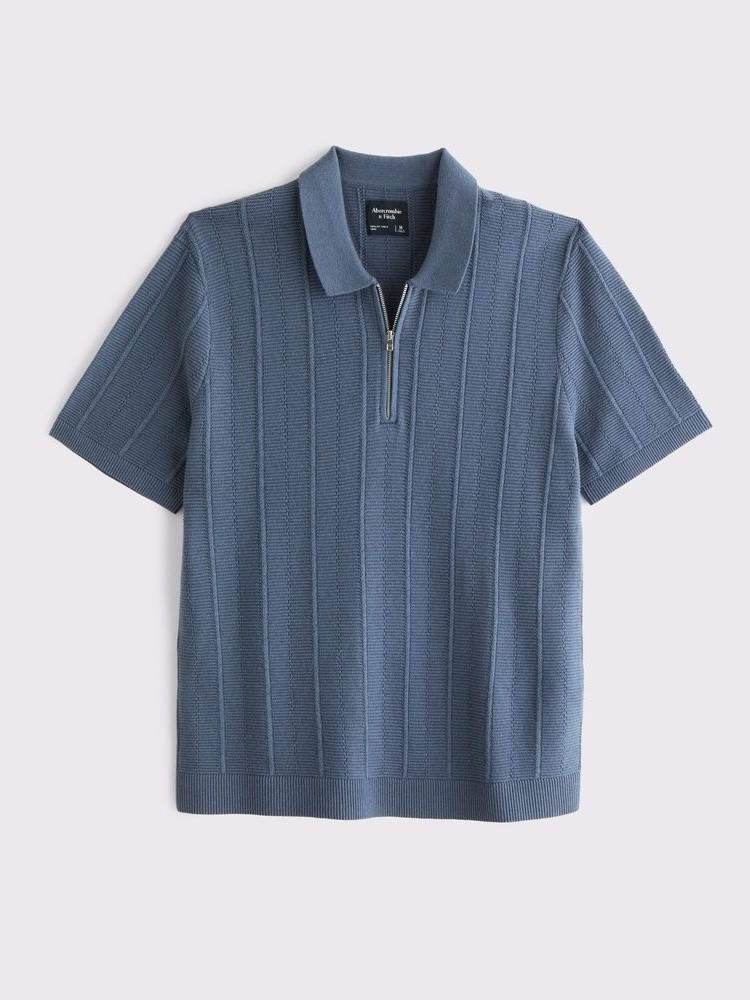
\includegraphics[height=5.6cm,keepaspectratio]{Images/vton/garment_upper.png}
        \par\smallskip
        \small (b) Trang phục phần trên
    \end{minipage}
    \begin{minipage}[t]{0.32\textwidth}
        \centering
        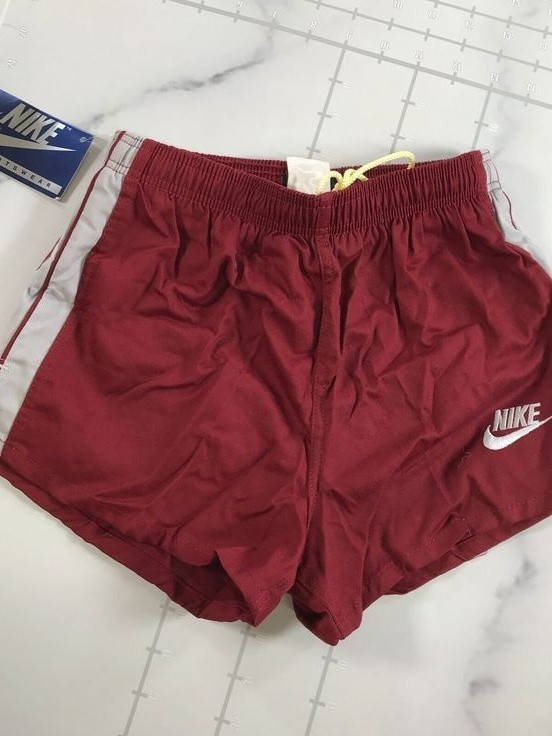
\includegraphics[height=5.6cm,keepaspectratio]{Images/vton/garment_lower.png}
        \par\smallskip
        \small (c) Trang phục phần dưới
    \end{minipage}
    \caption{Ảnh đầu vào cho thực nghiệm thử đồ ảo}
    \label{fig:vton-inputs}
\end{figure}

\medskip

CatVTON cục bộ được thực thi trên máy có GPU NVIDIA GeForce RTX 5060 với 8 GB VRAM, 16 GB RAM và CPU AMD Ryzen 9 8940HX. Mỗi bước sử dụng 25 vòng suy luận, \code{scale=2.5}, AutoMask và hậu xử lý repaint. Thời gian FLUX.2 được đo từ khi gửi yêu cầu tới Replicate đến khi nhận được ảnh kết quả.

\section{Kết quả thực nghiệm}

Hình~\ref{fig:vton-results} trình bày kết quả của hai phương án xử lý. CatVTON giữ ổn định khuôn mặt, tư thế, bàn tay và phần lớn bối cảnh gốc qua hai bước tuần tự. FLUX.2 tạo lại toàn bộ trang phục trong một lần xử lý, đồng thời thay đổi một số chi tiết về chất liệu áo, phụ kiện và đặc điểm hình ảnh.

\medskip

\begin{figure}[H]
    \centering
    \begin{minipage}[t]{0.32\textwidth}
        \centering
        
\includegraphics[height=6.4cm,keepaspectratio]{Images/vton/catvton_upper_result.png}
        \par\smallskip
        \small (a) CatVTON sau bước \code{upper}
    \end{minipage}
    \begin{minipage}[t]{0.32\textwidth}
        \centering
        
\includegraphics[height=6.4cm,keepaspectratio]{Images/vton/catvton_outfit_result.png}
        \par\smallskip
        \small (b) CatVTON sau bước \code{lower}
    \end{minipage}
    \begin{minipage}[t]{0.32\textwidth}
        \centering
        
\includegraphics[height=6.4cm,keepaspectratio]{Images/vton/flux2_outfit_result.png}
        \par\smallskip
        \small (c) Kết quả FLUX.2
    \end{minipage}
    \caption{Kết quả thử đồ của CatVTON cục bộ và FLUX.2 đám mây}
    \label{fig:vton-results}
\end{figure}

\medskip

Log xử lý cho thấy CatVTON hoàn thành bước thay trang phục phần trên trong khoảng 33 giây và bước thay trang phục phần dưới trong khoảng 31 giây. Tổng thời gian suy luận của chuỗi hai bước là khoảng 64 giây. Với cùng bộ ảnh tham chiếu, FLUX.2 trả kết quả toàn bộ trang phục sau khoảng 21 giây.

\medskip

\begin{table}[H]
\centering
\small
\caption{Thời gian xử lý Virtual Try-On trong thực nghiệm}
\label{tab:vton-observed-time}
\begin{tabularx}{\textwidth}{L{3.4cm}L{2.3cm}L{2.8cm}Y}
\toprule
\textbf{Phương án xử lý} & \textbf{Số bước} & \textbf{Thời gian} & \textbf{Đặc điểm} \\
\midrule
CatVTON phần trên & 25 vòng suy luận & Khoảng 33 giây & Tạo ảnh trung gian, giữ nguyên trang phục phần dưới. \\
\addlinespace
CatVTON phần dưới & 25 vòng suy luận & Khoảng 31 giây & Sử dụng ảnh kết quả của bước phần trên làm đầu vào. \\
\addlinespace
CatVTON toàn bộ trang phục & Hai bước tuần tự & Khoảng 64 giây & Tổng thời gian suy luận của hai bước. \\
\addlinespace
FLUX.2 toàn bộ trang phục & Một yêu cầu & Khoảng 21 giây & Xử lý đồng thời nhiều ảnh tham chiếu qua Replicate. \\
\bottomrule
\end{tabularx}
\end{table}

\section{Phân tích kết quả thực nghiệm}

Xét về thời gian xử lý, FLUX.2 hoàn thành toàn bộ trang phục nhanh hơn CatVTON hai bước khoảng 43 giây, tương ứng giảm gần 67\% thời gian so với chuỗi CatVTON. Chênh lệch này xuất phát chủ yếu từ cách tổ chức tác vụ: CatVTON phải thực hiện hai lần suy luận nối tiếp, trong khi FLUX.2 tiếp nhận nhiều ảnh tham chiếu trong một yêu cầu.

\medskip

Xét về mức độ bảo toàn ảnh gốc, CatVTON giữ khuôn mặt, tư thế, bàn tay, túi đeo và bối cảnh ổn định hơn. Bước thay phần dưới tiếp tục sử dụng kết quả của bước trước nên phần áo đã tạo được duy trì. Tuy nhiên, xử lý tuần tự làm tổng độ trễ tăng theo số vùng trang phục và có khả năng tích lũy sai lệch qua từng bước.

\medskip

FLUX.2 tạo kết quả có độ hoàn thiện thị giác cao và tái hiện rõ đặc điểm của quần tham chiếu, nhưng mô hình cũng thay đổi kết cấu áo, tỷ lệ cơ thể và một số chi tiết phụ kiện. Điều này phù hợp với bản chất của một mô hình sinh và chỉnh sửa ảnh tổng quát: kết quả có tính linh hoạt cao nhưng mức độ bảo toàn chính xác từng vùng ảnh khó kiểm soát hơn mô hình VTON chuyên biệt.

\medskip

Kết quả cho thấy hai phương án phù hợp với các mục tiêu khác nhau. CatVTON thích hợp khi cần chủ động dữ liệu, kiểm soát quá trình suy luận và giữ ổn định ảnh gốc. FLUX.2 phù hợp khi ưu tiên thời gian phản hồi và xử lý toàn bộ trang phục trong một yêu cầu. Việc hỗ trợ cả hai phương án giúp hệ thống lựa chọn theo điều kiện hạ tầng và yêu cầu trải nghiệm.

\section{Đánh giá kiến trúc}

Việc tách Medusa khỏi dịch vụ AI giúp các tác vụ sinh ảnh không chặn luồng thương mại điện tử. RabbitMQ tiếp nhận tác vụ VTON và giới hạn số thông điệp chưa xác nhận tại mỗi bộ tiêu thụ, nhờ đó tải xử lý phù hợp hơn với tài nguyên GPU. SSE hoàn thiện luồng bất đồng bộ bằng cách gửi trạng thái và ảnh kết quả về đúng giao diện đang chờ.

\medskip

Luồng AI Stylist sử dụng truy hồi trước khi sinh phương án phối đồ. Cách tổ chức này giới hạn tập sản phẩm mà mô hình được lựa chọn và cho phép Medusa kiểm tra lại dữ liệu giao dịch trước khi trả về giao diện. Mẫu thiết kế adapter tiếp tục giảm phụ thuộc trực tiếp vào Gemini, CatVTON hoặc Replicate, tạo điều kiện thay đổi mô hình mà không làm thay đổi toàn bộ luồng nghiệp vụ.

\medskip

Kiến trúc hiện tại đáp ứng mục tiêu của một bản triển khai kỹ thuật tối thiểu có nhiều thành phần tích hợp. Các ranh giới dịch vụ, hợp đồng dữ liệu và cơ chế xử lý bất đồng bộ đã được thể hiện trong mã nguồn và kết quả thực nghiệm. Tuy nhiên, để vận hành ở quy mô lớn hơn, hệ thống cần hoàn thiện bảo mật, độ tin cậy thông điệp và lưu trữ dùng chung.

\section{Hạn chế}

Cơ chế xác thực người dùng chưa hoàn chỉnh; một số API và giao diện vẫn sử dụng định danh mặc định. Luồng thanh toán mới mô phỏng quy trình Saga và đường dẫn gọi từ giao diện chưa thống nhất với API Medusa. Ảnh tải lên và ảnh kết quả VTON được lưu trên máy chạy dịch vụ, chưa sử dụng kho đối tượng dùng chung.

\medskip

Trong luồng VTON cục bộ nhiều bước, địa chỉ ảnh trang phục của tác vụ tiếp theo đang được lưu tạm trong trường \code{error_message}. RabbitMQ chưa có chính sách xử lý lại và hàng đợi thông điệp lỗi hoàn chỉnh; khi xử lý lỗi, thông điệp có thể được xác nhận để tránh lặp vô hạn. Dữ liệu \code{price} và \code{in_stock} trong LanceDB hiện sử dụng giá trị mặc định, vì vậy bộ lọc giá và tồn kho chưa phản ánh đầy đủ dữ liệu giao dịch từ Medusa.

\medskip

Thực nghiệm VTON sử dụng một bộ ảnh đầu vào và một lần đo cho mỗi phương án. Kết quả đủ để phân tích luồng xử lý và so sánh trong phạm vi đồ án, nhưng chưa đại diện cho biến động trên nhiều tư thế, loại trang phục, độ phân giải và điều kiện mạng. Hệ thống cũng chưa ghi nhận đầy đủ mối liên hệ từ phiên tư vấn hoặc tác vụ VTON tới hành động mua hàng.

\clearpage
